\subsection{Fit Sensitivity to Initialization}
Here we study the sensitivity of SFRESCO fitting to initial parameters. We used volume real and surface imaginary components of the optical potential only. Although there is improvement in the neutron scattering fit by inclusion of a spin-orbit imaginary term, optimal fits without this term are roughly 40\% of the fit with this additional term ($\chi^2/N = 3.310, 4.638 $). Optimal initial parameters were determined by successive fitting and reinitializing output parameters until a stable minimum was achieved with parameters comparable to the initial global potential fits from \cite{capote2009ripl}.
\par
In Figure \ref{fig:initializations} below, we plot the SFRESCO $\chi^2/N$ fit error against modifications of a single parameterization. To overlay dissimilar parameter values, the plotted input parameter is normalized by its determined optimized value. $\chi^2/N$ as a choice of parameter of interest (as opposed to the output value of the varied parameter) was from the observation that  $\chi^2/N$ correlates strongly with optical potential parameters approaching the optimal fit values within a few percent. From Fig \ref{fig:pnV}, we see that initializations to both depth parameters for protons and neutrons arrive at optimum for roughly $\pm$50\% of optimal values. From Fig. \ref{fig:pnr}, While not as centered around $\frac{P_{in}}{P_{optimal}}=1$ as the depth parameters, the radius parameters appear to converge for roughly $\pm$25\% of optimal values. In Fig. \ref{fig:pna}, we demonstrate that diffuseness is potentially the most convergent parameter (see neutron surface imaginary converge for $\pm$100\% of the optimal value), diffuseness is the least consistent parameter. The worst demonstrated convergence is the proton surface imaginary diffuseness, which converges for $\frac{P_{in}}{P_{optimal}}=1.0-0.0+0.5$.
\par
Two peculiarities were discovered while spanning these parameters.
\begin{enumerate}
\item Multiple initializations regions of the proton real volume depth lead to optimal parameterization. Fig. \ref{fig:pnV} shows how $V_0\approx 0$ gives results consistent with $V_0 \approx V_{optimal}$ while the region $0.1 \leq \frac{V_0}{V_{optimal}} \leq 0.6$ returns a significantly worse fit.
\item It is important to stress the value of repeated, varied initialization over a range of initializations deemed reasonable for a parameter. See the neutron real volume depth $\frac{V_0}{V_{optimal}} = 0.55 \pm <0.05$. This region of poorer $\chi^2$ metric sits in a region of more optimal parameter finding, and is relatively narrow ($<$ 3 MeV). Given the approximate nature of the global potentials that were used to arrive at optimal fitting parameters, this narrow window and so a range of initial values (centered around the global parameter fit) ought to be considered. 
\end{enumerate}
    \begin{figure}[h]
    \begin{subfigure}{0.5\textwidth}
    
		\centering
		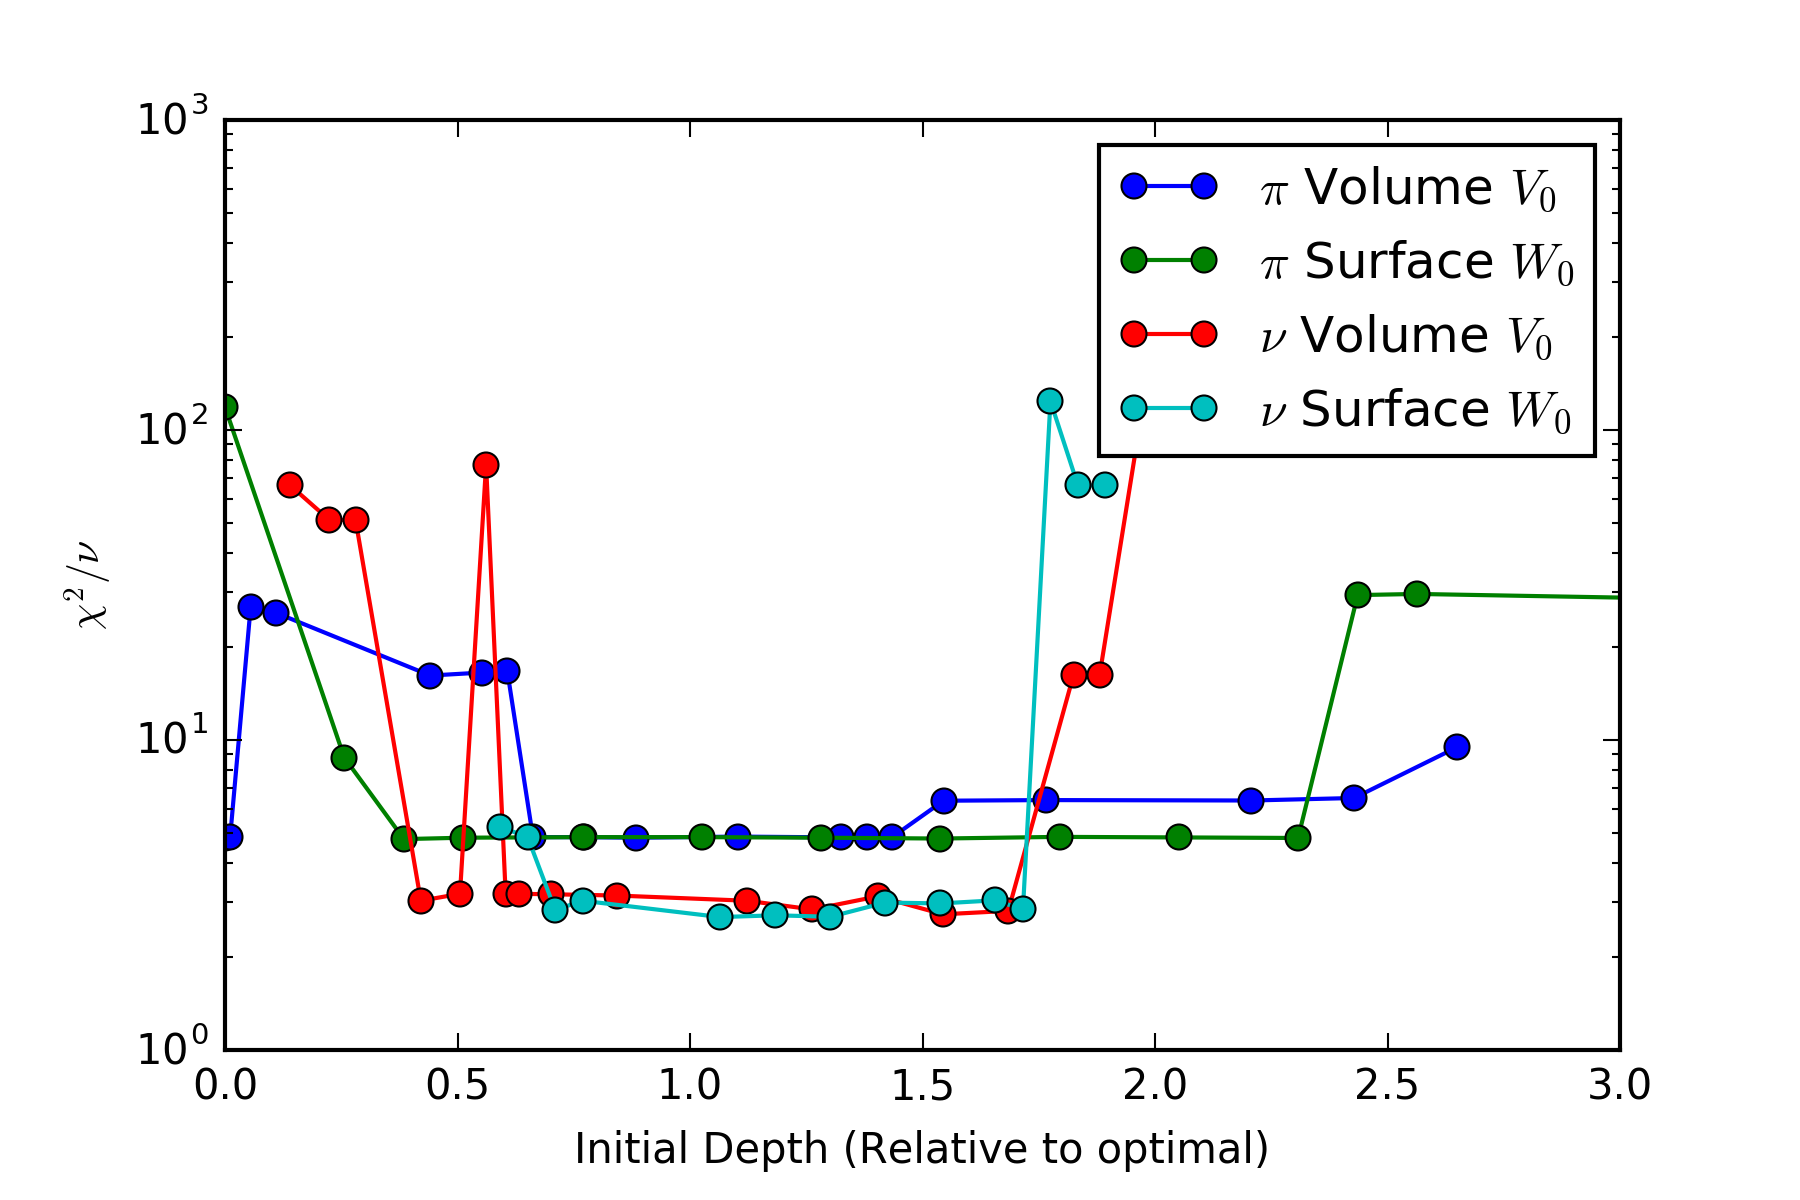
\includegraphics[width=0.98\textwidth]{pnV.png}
		\caption{Optical potential depth parameters }
		\label{fig:pnV}
	\end{subfigure}
        \begin{subfigure}{0.5\textwidth}
		\centering
		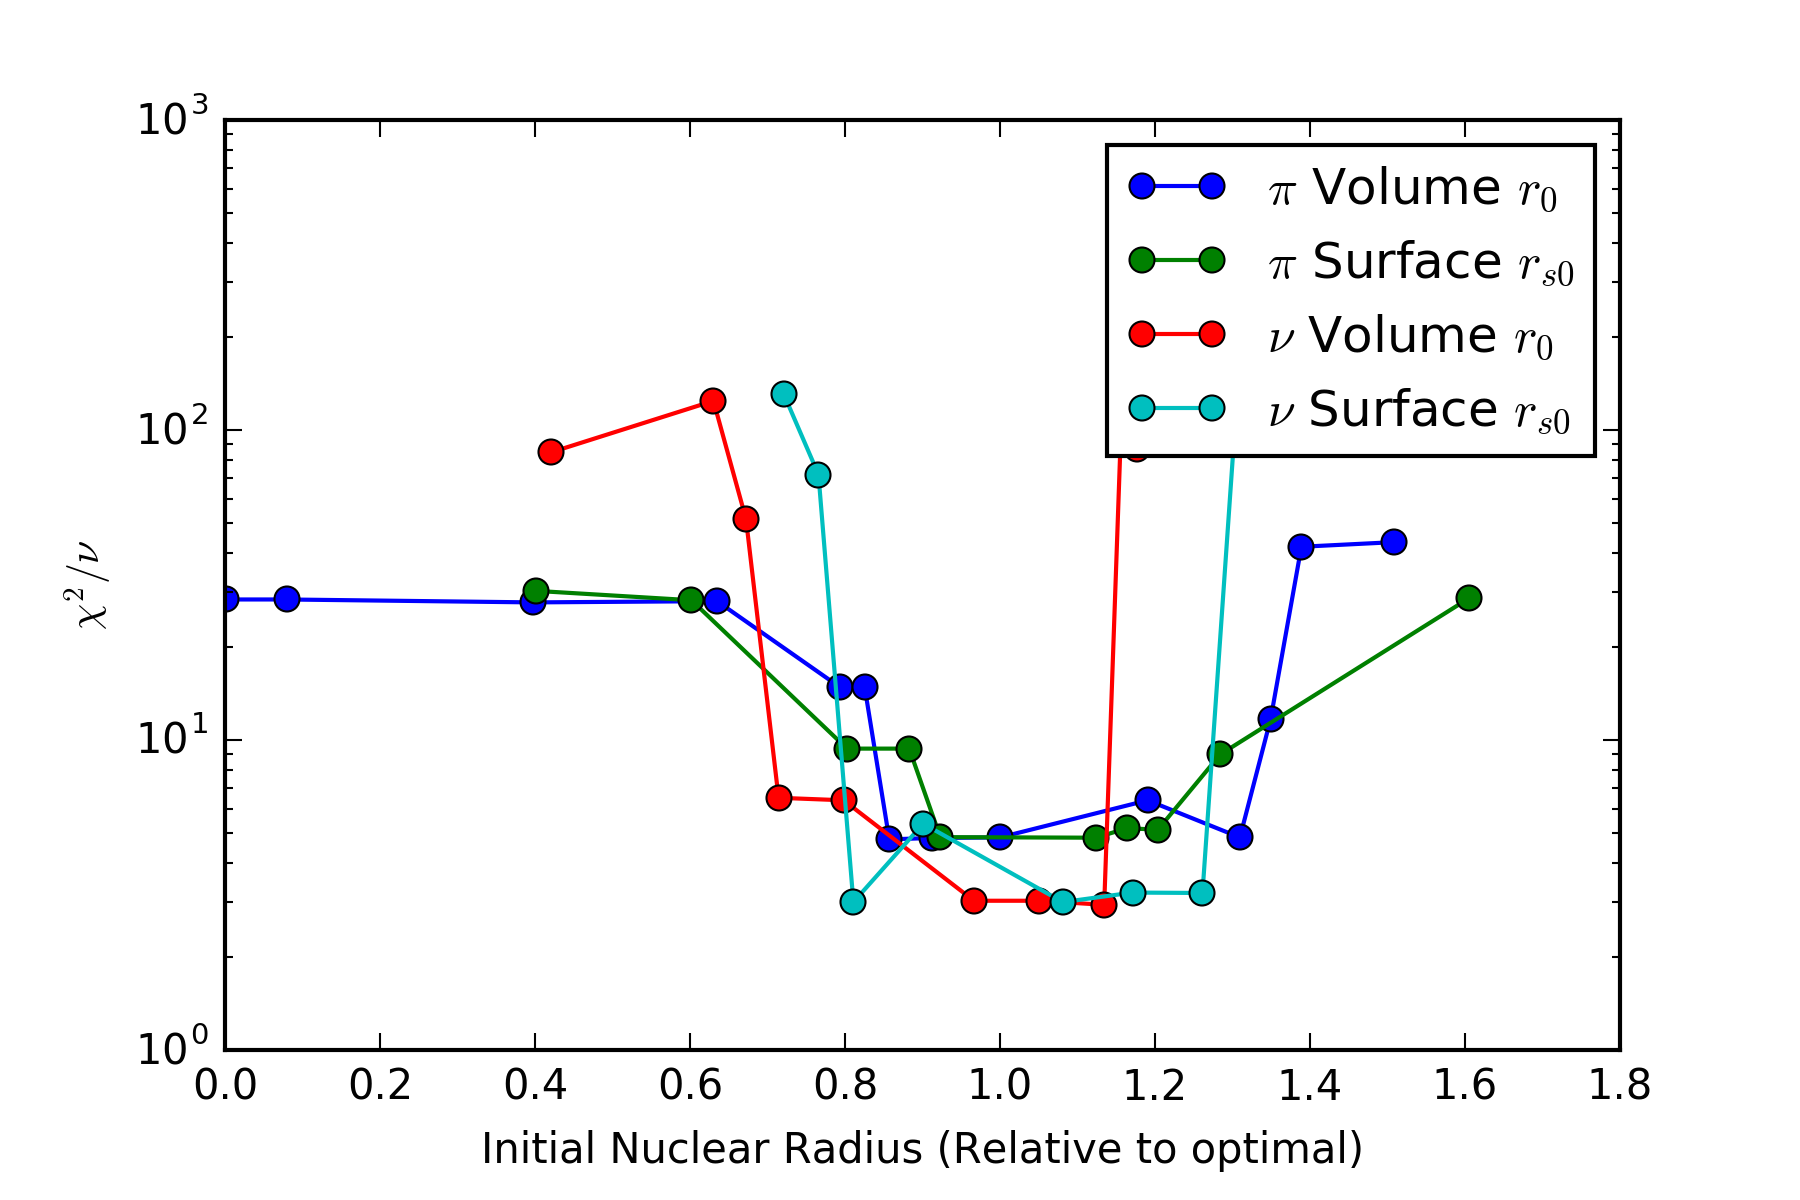
\includegraphics[width=0.98\textwidth]{pnr.png}
		\caption{Nuclear radius parameters }
		\label{fig:pnr}
        \end{subfigure}
        \begin{subfigure}{0.5\textwidth}
		\centering
		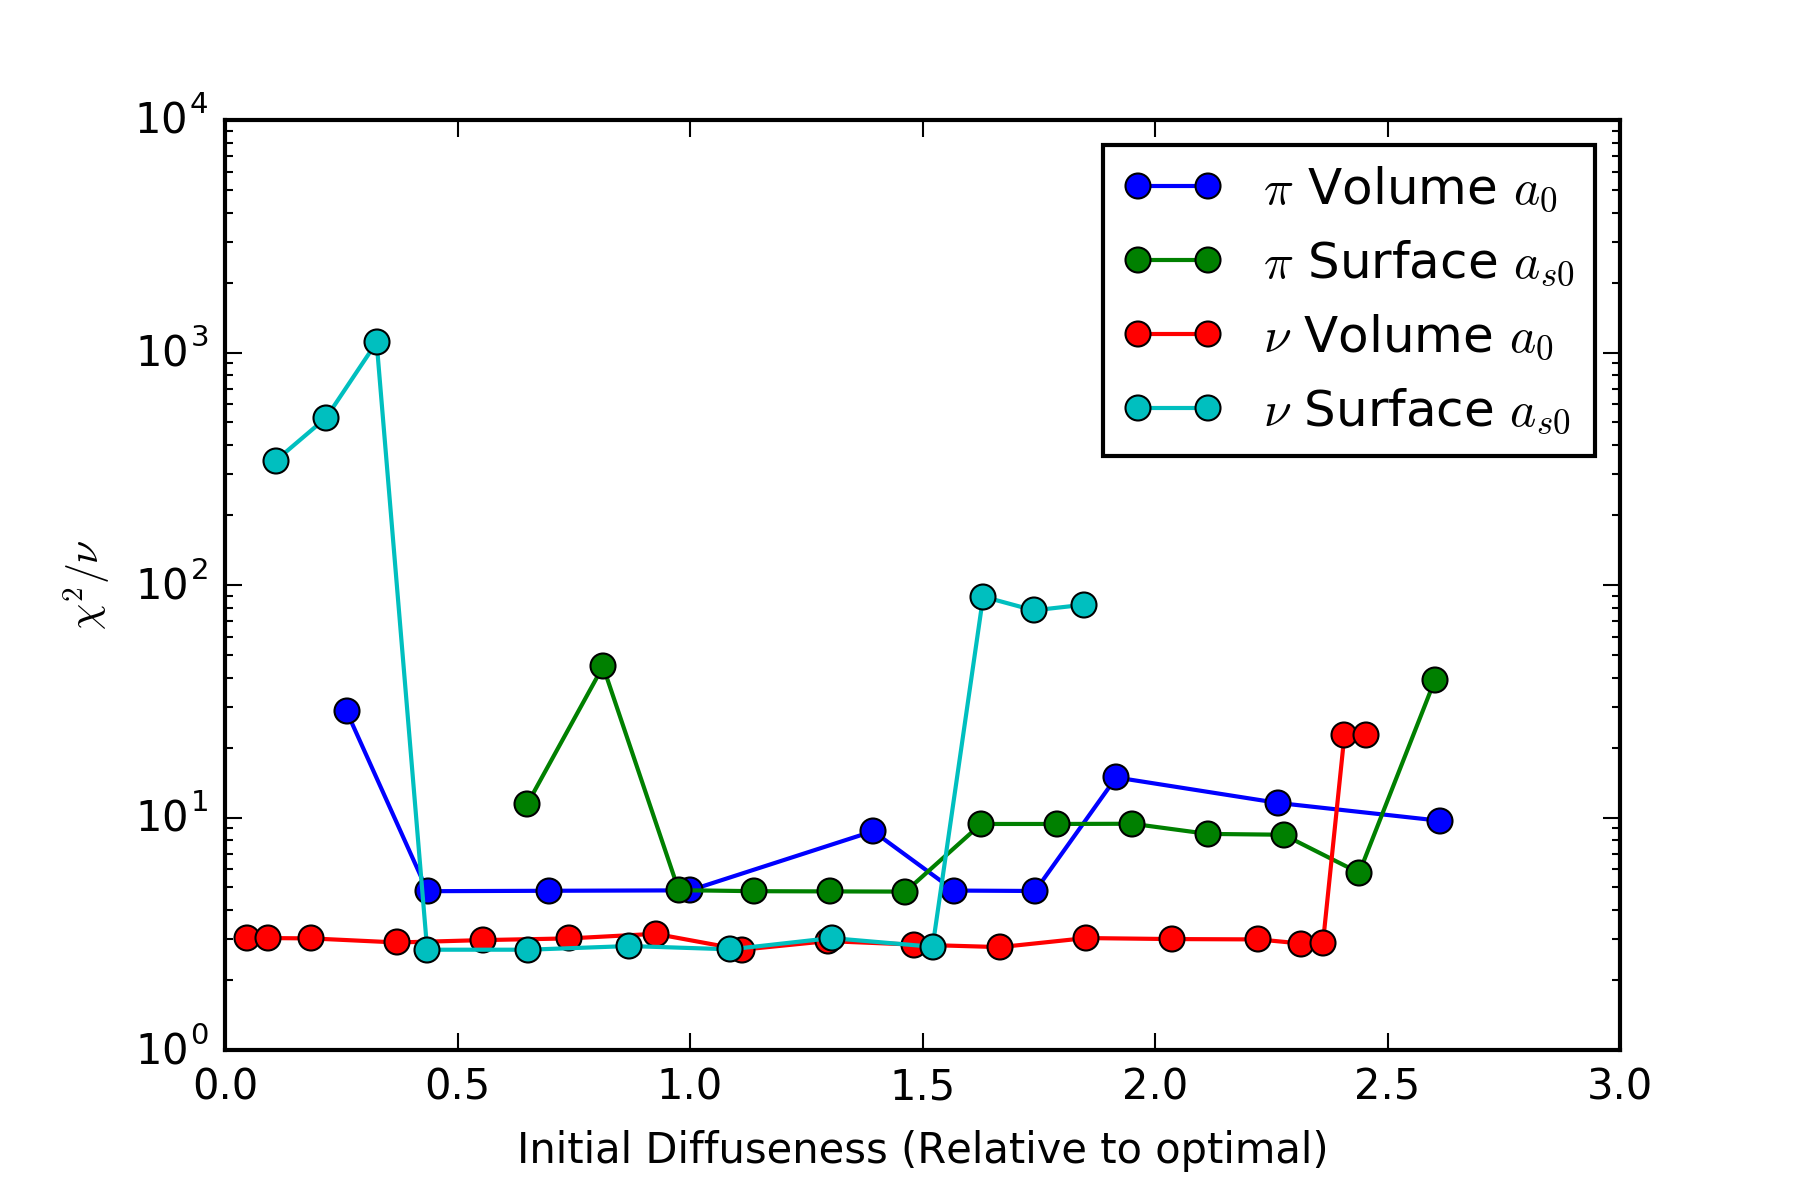
\includegraphics[width=0.98\textwidth]{pna.png}
		\caption{Nuclear diffuseness parameters  }
		\label{fig:pna}
        \end{subfigure}
        \caption{Measure of error of SFRESCO fits for different initial parameterization of the depth part of the optical potential for 49.35 MeV protons ($\pi$) and 40 MeV neutrons ($\nu$) scattering on $^{208}$Pb. Plotted on the x-axis is the ratio of $\frac{P_{initial}}{P_{optimal}}$. }
        \label{fig:initializations}
	\end{figure}
